

\chapter{Conclusion}

\label{chap:conclusion} 
\newcommand{\toolname}{TypeTutor}



\graphicspath{{Figures/Conclusion}}

In this thesis, we started by establishing the context of our work in the field statically-typed programming language. The studies and systems we contribute focus on the Haskell programming language, but there are plenty opportunities to extend our findings to broader and more mainstream programming languages as well. We then proceeded to give a brief introduction to type checking based on constraint satisfiability. Using the notions in constraint logic, we proposed a categorization of type error. We then showed three projects, each with its own research focus and technical contributions.


\section{Contributions}


\subsection{A categorization of type errors based on the structure of the evidence of a type error}

Based on how type errors are perceived by human programmers and the theories in constraint satisfiability research, we put forward a categorization of type errors. This categorization aims to charactorize 3 important features of type errors that help deciding how to best report them. 


With this classification, we explored the three main systems we developed --  Chameleon (Chapter \ref{chap:chameleon}), Goanna (Chapter~\ref{chap:goanna}), and GeckoGraph (Chapter~\ref{chap:gecko-graph}) -- to address the challenges of type error debugging in different error categories.

\subsection{Explaining Multi-step type erros and the chain of thought visualization}

\subsubsection{Technical Contribution - Chameleon}
We contribute Chameleon, an interactive Haskell type error debugging tool. Internally, Chameleon computes all relevant locations that contribute to the type of error. Via a set of iteratively designed interface, Chameleon preserves the two alternatives of the type error and the supporting evidence for each.

\subsubsection{How programmers use type error slicing and chain of thought visualization to understand type errors}
We  contributed a series of studies of the effects of debugging with visual representation of types and interactively explored type errors. We show that there is a difference between using traditional tools and enhanced type error debugging tools like Chameleon. And we show that this difference is more significant when debugging complex type errors.

\subsection{Iterate potential causes of multi-wintness and multi-party errors}

\subsubsection{Technical Contribution -- Goanna}

We contribute Goanna, a Haskell type error debugging tool. 

Like Chameleon, Goanna iterates relevant locations that contribute to the type error and presents alternatives to the type error. 

Different from Chameleon, Goanna will exhaust all possible alternative explanations of the type error. Also, Goanna presents a type error by dividing it into a list of potential causes and their respective fixes. With Goanna, Haskell programmers can resolve type errors by exploring a list of potential error root causes. These causes are ordered using our heuristics so that the more likely causes are on top. We show that via our empirical evaluation that Goanna outperforms existing Haskell compilers when explaining the type error, with the slight disadvantage of an increased computation time.

\subsubsection{An evaluation on accuracy, conciesness and performance of MCS-based type debugging and our heuristics}

We evaluated Goanna's effectiveness using 86 diverse Haskell programs from online discourse, demonstrating its ability to accurately identify and resolve type errors. Additionally, we present a collection of techniques and heuristics to enhance Goanna's suggestion-based error diagnosis and show their effectiveness from our evaluation.


\subsection{Visualizing Types}

\subsubsection{Technical Contribution -- GeckoGraph}

In addition to the two systems, I also contribute GeckoGraph, a graphic notation for Haskell types. GeckoGraph describes the same information as a type signature does, but uses colours, shapes, and symbols to make certain structures easy to identify at a glance. GeckoGraph is designed to use visual elements to improve the understanding of type-level concepts. This includes type classes, parametric type variables, and high-rank types. When used to compare two types, GeckoGraph helps clarify differences visually. It makes errors like too few or too many arguments in applications, unmet type class constraints obvious.

\subsubsection{An evaluation on how programmers use diagramtic type notation}

We conducted a large-scale study on the effectiveness of using GeckoGraph to perform a series of Haskell tasks. We concluded that with GeckoGraph, programmers are able to succeed in harder tasks.

\section{Future Work}

From the work presented in this thesis, we generalize the tasks of debugging type errors and our proposed debugging techniques in a few idiomatic interations.  Such as the interactive debugging steps in Chameleon, and error cause exploration in Goanna. Although resides in different system, these user interaction idioms work together to complement each other. Therefore, we envision that an useful future work direction is to re-imagine the debugging workflow and leverage on all the proven useful techniques from Chameleon, Goanna and GeckoGraph.

\subsection{Future Directions of Type Debugging Tool}

I devised a Type-Driven Debugging Extension that compatible with underlying type checking tools such as Chameleon and Goanna.  It integrate the, it adaptively show a minimal diagonisis of the type error and allow users to interactively query part of the reasoning behind this type judgement.  

\subsection{Question-based Type Debugging}
Many research show positive impact from natual debugging interface, that is,  framing the debugging tasks into questions that align with programmers objective. However, most experimentation in this direction are all focusing on debugging runtime errors. The narrowed focus on runtime error can be attributed to the fact that type level debugging often cannot provide enough meaning anlaysis. This has changed in the last decade or so. With the improvement in our debugging information, I have envisioned a form of quation-based type debugging interface that answers to common debugging motif. 

\subsection{Why questions}
In The tool
\begin{figure}[hbt]
  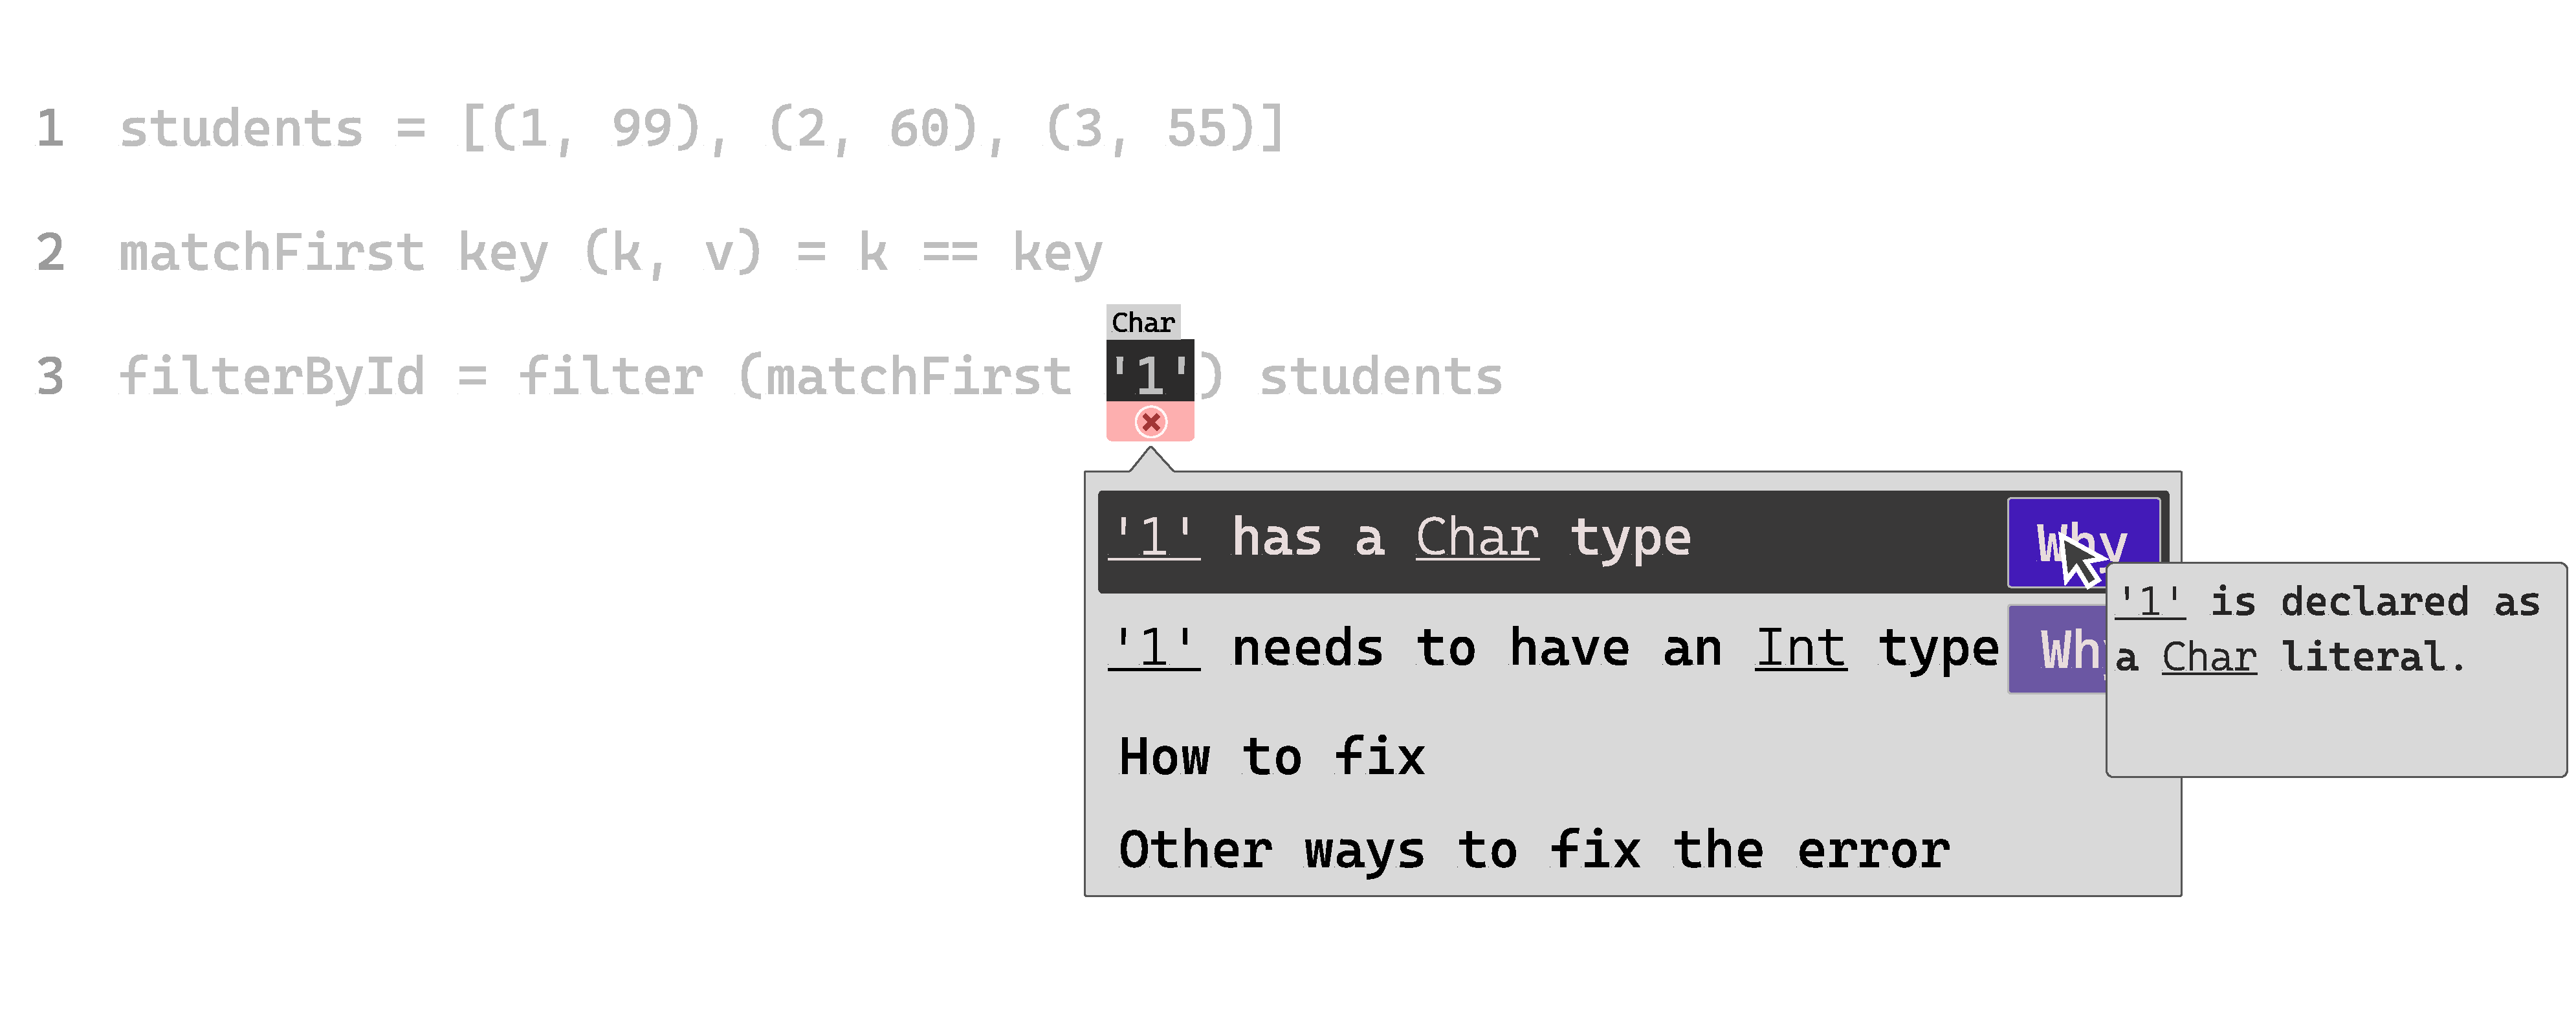
\includegraphics[width=\linewidth]{ExplainError1.pdf}
  \caption{
      Displaying a type error in level 1 explanation
    }
\end{figure}


\begin{figure}[hbt]
  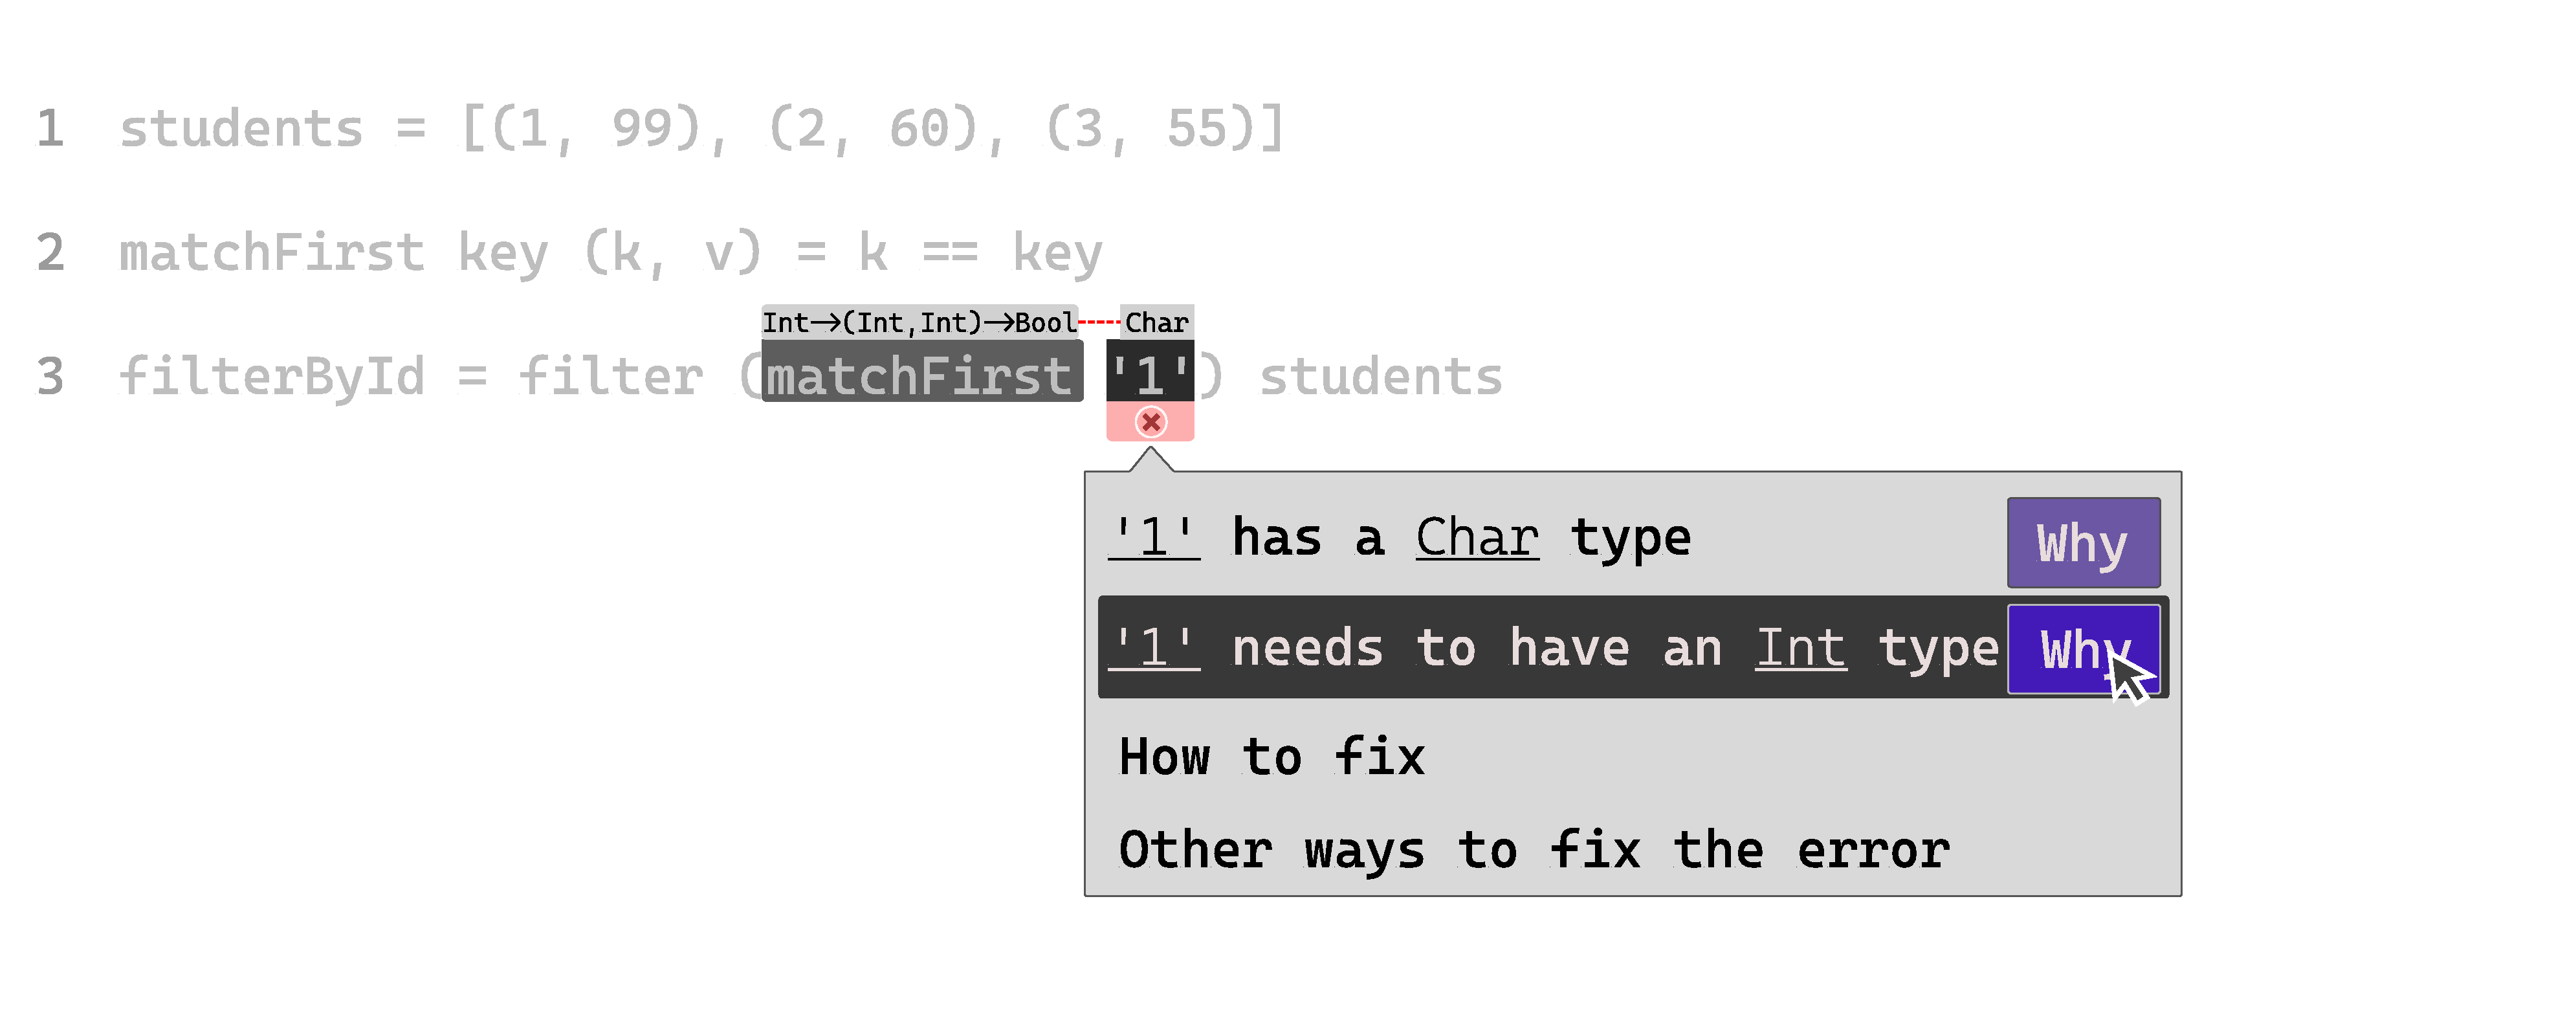
\includegraphics[width=\linewidth]{ExplainError2.pdf}
  \caption{
      Displaying a type error in level 1 explanation
    }
\end{figure}


\begin{figure}[hbt]
  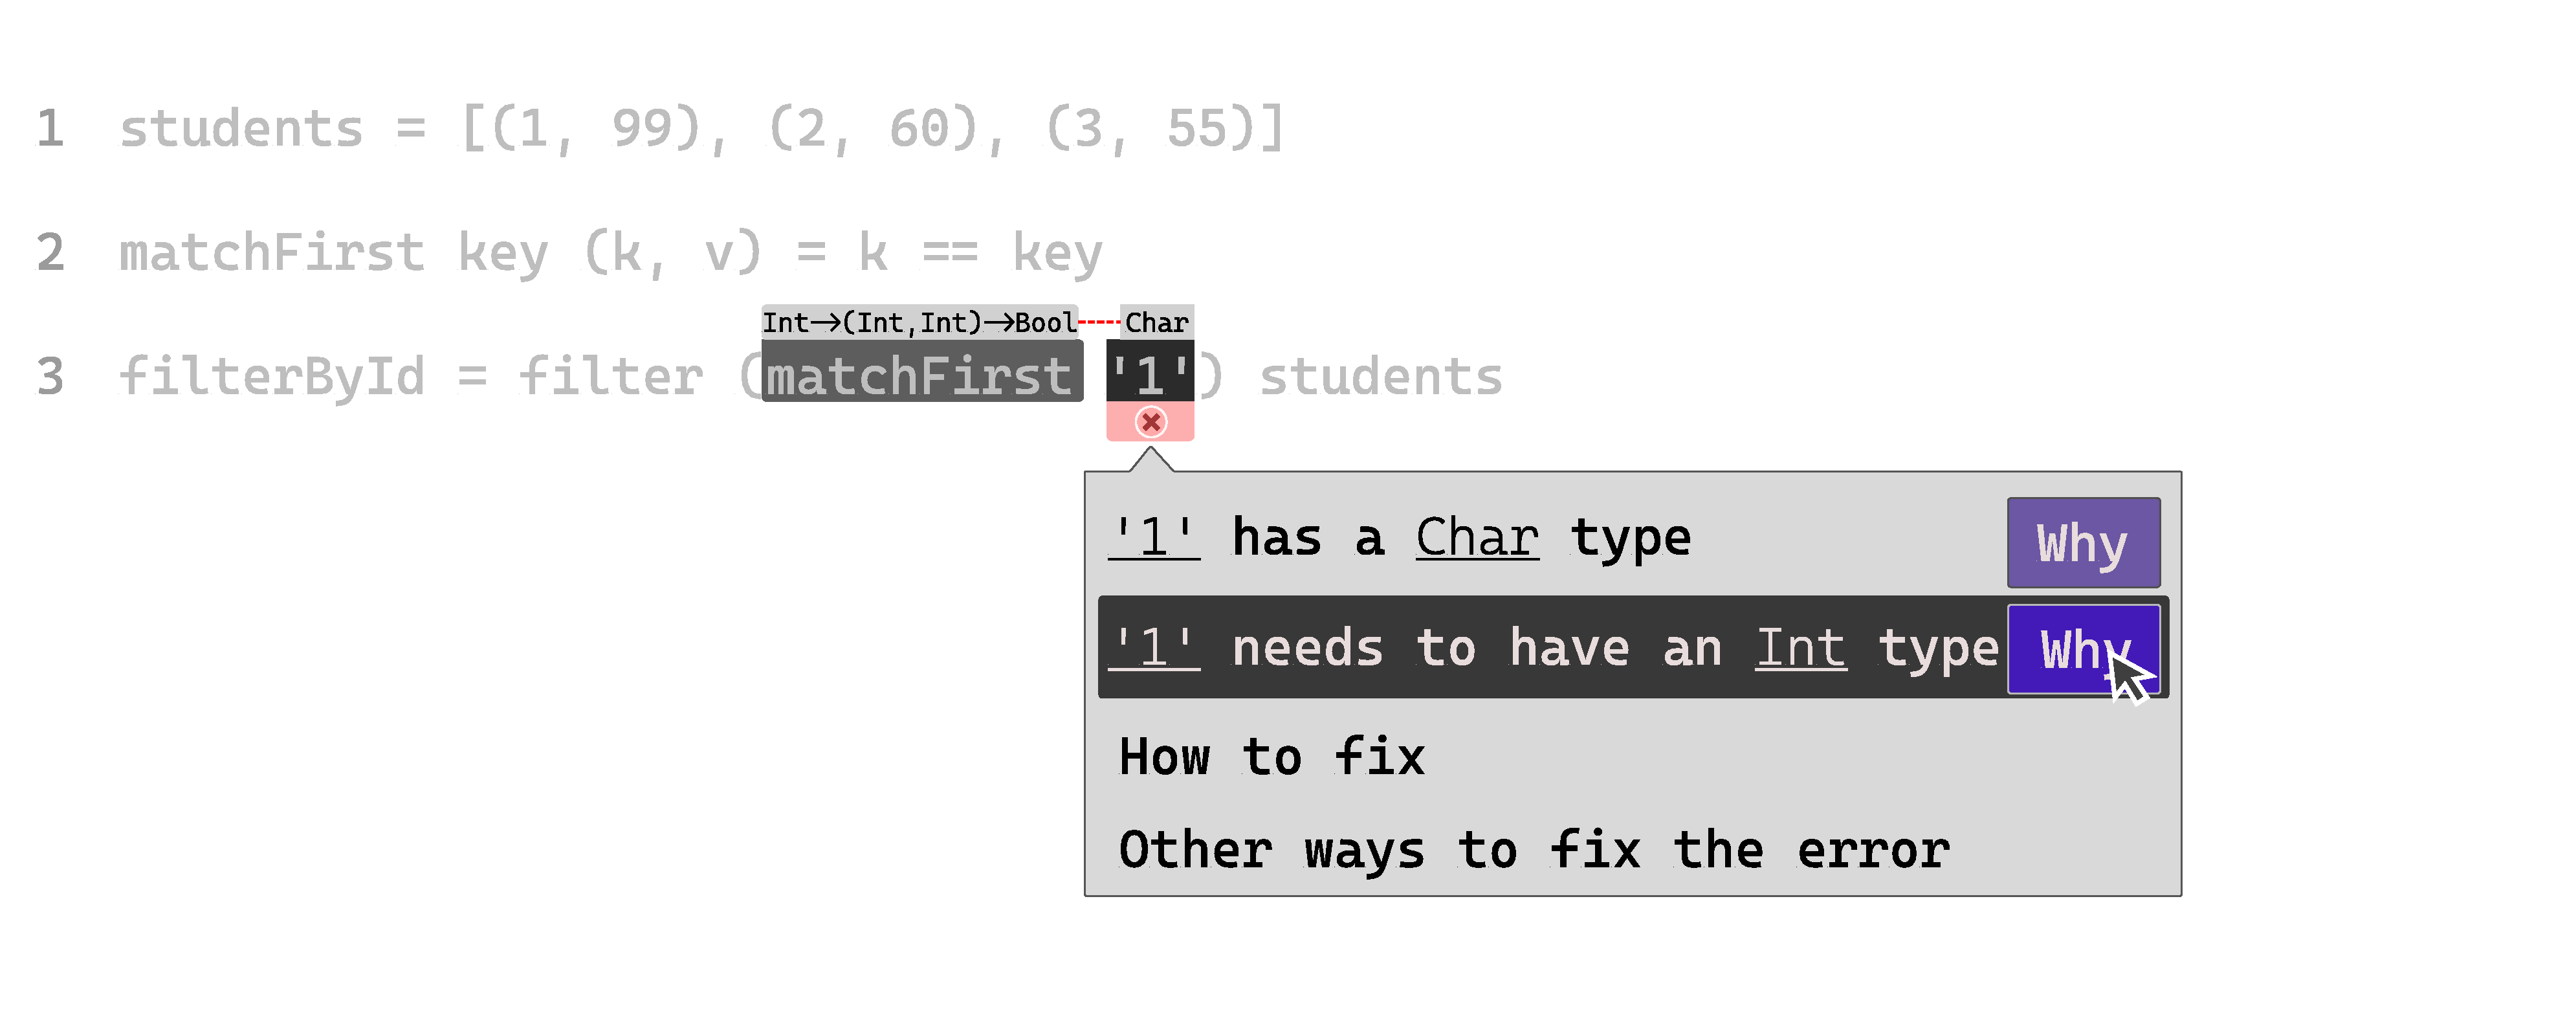
\includegraphics[width=\linewidth]{ExplainError2.pdf}
  \caption{
      Displaying a type error in level 1 explanation
    }
\end{figure}
\subsection{Support for Other Languages}
\subsubsection{Motivation}
While Haskell is useful platform for studying programming languages and type systems, it is not the only one that benefit from static type systems. It is in fact very common for programming languages to suffers from usability issues in the pursuit for advanced and strict type checking. In practice, many programmers find the TypeScript and Rust equally confusing with the amount of type level programming facilited in the language and the lack of proper tools to interpret them. Therefore, it will be an exiting next step to migrate the techniques and concepts in this work to other statically typed programming languages. 

\subsubsection{Feasibility}

One advantage of our work in type debugging systems and tools is that the theories and techniques are transferreable to other languages.  

For the systems like Chameleon and Goanna, the generation is specific to the language but the constraint satisfiability solving is general enough to be replaced with other systems. The MUS/MCS enuemeration is general library that can work with any constraint system. The visualization of MUS and MCS is also adaptable given that they are only highlights slices in the source code.

For system like GeckoGraph, the basic construction rules of GeckoGraph algebraic data types, type classes, bounded quatification, and parametric polymorphism. These type systems ideas are universal among many language. That said, GeckoGraph is not suited for type systems that heavily lean on norminal types. For a system like Java where norminal types are widely used, and tying relations are framed in the inheritance, visualizations such like class diagram are more suited. 



\subsubsection{Challenges}

For the systems like Chameleon and Goanna, only two challenges to be solved. First is implementing the constraint generation. Because this is the only part that differs from language to language. Once the typing relations are interpreted in constraint languages, the rest is all language agnositic.  Second is to handle the intricacy of informing programmers where the type constraints are generated from the source code. Traditionally this is always done by highligts. But this takes the assumpiion that 


\section{Final words}

This research was centered around two key questions: what are the specific tasks when dealing with type errors, and how can we improve interaction with them? From this work, we have proposed a novel classification of type errors, revealing that each category comes with its unique set of challenges. This has resulted in three distinct fields of exploration. 

This research, grounded in a human-centered approach, demonstrates promising methods to improve the way we interact with static type systems within contemporary programming environments. It provides a basis for future research in the field of type error debugging and paves the way for the development of new programming tools centered on simplifying the challenges of debugging type errors. 
